\section{ Comparison of models}\label{model_comparisons}

As mentioned in Section \ref{cnn_ref}, we used a Keras Tuner model to find the hyperparameters that would yield the highest accuracy.
Instead of hard-coding hyperparameters when building a model with Keras API, we defined a search space of possible values with \verb|HyperParameter| class, and used that as a hyperparameter.

We passed the created model to a \verb|RandomSearch| class, with a few other parameters, such as batch size, number of epochs and maximum number of trials.
As we started the hyperparameter search, Keras Tuner started picking a selected set of hyperparameters randomly, which were used to train a model.
This process was repeated a number of times.
The used hyperparameters and achieved accuracy on the validation set for each trained model were logged in a text file for later use.

After training several different models we picked a few and compared them.
Comparison of models trained in Edge Impulse Studio was also done.

To distinguish models from one another we decided to mark them with a number and letters \textit{a}, \textit{b}, \textit{ei} and \textit{tl}.
Models with letters \textit{a} and \textit{b} were trained using our system.
Models marked with \textit{ei} and \textit{tl} were created in the Edge Impulse Studio.
More specifically, \textit{ei} models have a same basic CNN architecture as our models, while \textit{tl} models were trained by the Transfer Learning technique, which reuses a pre-trained MobileNetV2 architecture.
The Tables that are shown below list one of the metrics as accuracy.
By accuracy we mean validation accuracy; it tells us how well the model performed on a validation dataset.

\subsection{ Hyperparameter search space and result's analysis}

The general structure of the CNN model was already described in Section \ref{cnn_ref} and in Figure \ref{model_code}.
We decided to search for the following hyperparameters: 

\begin{itemize}
    \item Number of filters in all three convolutional layers (can be different for each layer)
    \item Size of filters in all three convolutional layers (same for all layers)
    \item Size of the dense layer
    \item Dropout rate 
    \item Learning rate
\end{itemize}

The possible values of hyperparameters (also known as a hyperparameter search space) are specified in Table \ref{hyper_table1}.
\newline
\begin{table}[ht]
    \centering
    \caption{ First hyperparameter search space}
    \rowcolors{2}{white}{gray!25}
    \begin{tabular}{@{} *5l @{}}    \toprule
        \textbf{Hyperparameter} & \textbf{Set of values}\\\midrule
        \verb|FilterNum1|       & From 16 to 80, with a step of 8\\ 
        \verb|FilterNum2|       & From 16 to 80, with a step of 8\\ 
        \verb|FilterNum3|       & From 16 to 80, with a step of 8\\
        \verb|FilterSize|       & 3 x 3 or 3 x 4\\
        \verb|DenseSize|        & From 16 to 96, with a step of 8\\
        \verb|DropoutRate|      & From 0.2 to 0.5, with a step of 0.05\\
        \verb|LearningRate|     & 0.0001 or 0.0003\\\toprule
        \textbf{Random search}  & \textbf{value}\\
        \textbf{variable}       & \\\midrule
        \verb|EPOCHS|           & 25\\
        \verb|BATCH_SIZE|       & 100\\
        \verb|MAX_TRIALS|       & 300\\\bottomrule
    \end{tabular}
    \label{hyper_table1}
\end{table}

The search spaces of \verb|FilterNumX|, \verb|DenseSize| and \verb|DropoutRate| hyperparameters were chosen based on initial training tests conducted on a thermal image dataset and other various models that were trained on similar data.
The value of \verb|FilterSize| is usually 3 x 3; however, most of the example ML projects that we could find on the Internet were training on image data of the same dimensions.
We wanted to test how a filter with the same ratio of dimensions as image data (3 x 4 and 60 x 80 respectively) would perform.
The hyperparameter \verb|learning_rate| was chosen heuristically; we saw that 10 times higher values, such as 0.001 or 0.003, would leave the model's accuracy stuck at suboptimal optima, from where it could not be improved anymore.

We also had to set 3 variables that affected directly how long the random search would last.
From initial tests we saw that models usually reached maximum possible accuracy at around the \nth{20} epoch, so, to give some headroom we set the number of epochs to 25.
We kept the batch size relatively small, at 100, which meant that weights would get updated regularly.
The \verb|MAX_TRIALS| hyperparameter had the biggest impact on the training time, so we set it to 300.

The training lasted for about 12 hours. 
After it was done we compiled a list of all 300 trained models and their different hyperparameter values, number of parameters and achieved accuracies.
Part of it can be seen in Table \ref{hyper_results1}.

After analysing results we came to several conclusions:

\begin{enumerate}
    \item We saw that almost all trained models, except for the last one, achieved accuracy above 90 \%. This proved that the general architecture of the model was appropriate for the problem.
    \item We could not see any visible correlation between a specific choice of a certain hyperparameter and accuracy. This showed that selection of hyperparameters is a non-heuristic task, at least for our particular problem.
    \item Filter of size 3 x 4 did not perform significantly better compared to one with size 3 x 3. 
    \item The first 200 models covered an accuracy range of 0.62 \%. However, inside of this range, the number of parameters varied hugely, for example, the model \textit{192a} had more than 8 times fewer parameters than the model \textit{96a}, although the difference in accuracy (0.27 \%) was negligible.
\newline
\end{enumerate}
\begin{table}[ht]
    \centering
    \caption{ Partial results of the first random search of hyperparameters}
    \rowcolors{2}{gray!25}{white}
    \begin{tabular}{llllllllrl}
    \textbf{Model ID} & \rot{FilterNum1} & \rot{FilterNum2} & \rot{FilterNum3} & \rot{DenseSize} & \rot{DropoutRate}  &\rot{FilterSize} & \rot{LearningRate} & \rotatebox{45}{\parbox{2cm}{Number of parameters}} & \rot{Accuracy[\%]}  \\\toprule
        0a & 72 & 80 & 64 & 72 & 0.4  & 3x4 & 0.0003 & 1,514,400 & 98.35\\
        1a & 32 & 40 & 72 & 56 & 0.35 & 3x4 & 0.0001 & 1,260,332 & 98.31\\
        2a & 40 & 48 & 32 & 64 & 0.35 & 3x4 & 0.0001 &   656,797 & 98.31\\
        3a & 56 & 16 & 48 & 72 & 0.4  & 3x4 & 0.0001 & 1,057,924 & 98.28\\
        4a & 80 & 64 & 40 & 96 & 0.45 & 3x4 & 0.0003 & 1,245,788 & 98.28\\\midrule
       96a & 16 & 32 & 72 & 80 & 0.25 & 3x4 & 0.0001 & 1,762,508 & 98.00\\
       97a & 72 & 56 & 40 & 56 & 0.45 & 3x4 & 0.0003 &   748,580 & 98.00\\
       98a & 32 & 24 & 24 & 48 & 0.35 & 3x3 & 0.0001 &   358,308 & 98.00\\
       99a & 48 & 16 & 40 & 40 & 0.45 & 3x3 & 0.0003 &   493,412 & 98.00\\
      100a & 24 & 72 & 64 & 40 & 0.45 & 3x3 & 0.0003 &   844,684 & 98.00\\\midrule
      191a & 64 & 56 & 16 & 52 & 0.4  & 3x3 & 0.0001 &   386,996 & 97.76\\
      192a & 48 & 40 & 24 & 24 & 0.4  & 3x4 & 0.0001 &   208,172 & 97.73\\
      193a & 56 & 64 & 72 & 24 & 0.25 & 3x4 & 0.0003 &   617,692 & 97.73\\
      194a & 48 & 72 & 48 & 32 & 0.25 & 3x4 & 0.0003 &   544,652 & 97.73\\\midrule
      295a & 48 & 32 & 64 & 16 & 0.5  & 3x4 & 0.0001 &   351,012 & 95.87\\
      296a & 40 & 24 & 56 & 24 & 0.5  & 3x4 & 0.0001 &   431,572 & 95.77\\
      297a & 56 & 16 & 80 & 16 & 0.2  & 3x4 & 0.0001 &   411,020 & 95.63\\
      298a & 24 & 16 & 48 & 24 & 0.5  & 3x4 & 0.0001 &   359,924 & 94.46\\
      299a & 40 & 48 & 56 & 16 & 0.35 & 3x3 & 0.0003 &   310,860 & 82.86\\\bottomrule
    \end{tabular}
    \label{hyper_results1}
\end{table}
It was apparent from the results that large models were not necessary to achieve high accuracy, so we decided to run the random search of hyperparameters again.
This time we lowered the maximum and the minimum numbers of filters and size of the dense layer.
We decreased all steps from 8 to 2, thus increasing the number of possible configurations.
We decided to lower the bottom boundary of \verb|DropoutRate| from 0.2 to 0.0, which meant that some models would not be using the dropout layer at all.
We expected that training without the dropout layer would produce suboptimal results, however, we wanted to test it.
The redefined search space for the second random search can be seen in Table \ref{hyper_table2}
We increased the number of \verb|MAX_TRIALS| from 300 to 500, as we were expecting that more models would end up underfitting, and also because there would be more possible options because of the smaller step size.
\newline
Partial results of the random hyperparameter search can be seen in Table \ref{hyper_results2}.
\newline
\begin{table}[ht]
    \centering
    \caption{ Second hyperparameter search space}
    \rowcolors{2}{white}{gray!25}
    \begin{tabular}{@{} *5l @{}}    \toprule
        \textbf{Hyperparameter} & \textbf{Set of values}\\\midrule
        \verb|FilterNum1|       & From 4 to 48, with a step of 2\\ 
        \verb|FilterNum2|       & From 4 to 48, with a step of 2\\ 
        \verb|FilterNum3|       & From 4 to 48, with a step of 2\\
        \verb|FilterSize|       & 3 x 3 or 3 x 4\\
        \verb|DenseSize|        & From 4 to 48, with a step of 2\\
        \verb|DropoutRate|      & From 0.0 to 0.5, with a step of 0.05\\
        \verb|LearningRate|     & 0.0001 or 0.0003\\\toprule
        \textbf{Random search}  & \textbf{value}\\
        \textbf{variable}       & \\\midrule
        \verb|EPOCHS|           & 25\\
        \verb|BATCH_SIZE|       & 100\\
        \verb|MAX_TRIALS|       & 500\\\bottomrule
    \end{tabular}
    \label{hyper_table2}
\end{table}
\begin{table}[ht]
    \centering
    \caption{ Partial results of the second random search of hyperparameters}
    \rowcolors{2}{gray!25}{white}
    \begin{tabular}{llllllllrl}
    \textbf{Model ID} & \rot{FilterNum1} & \rot{FilterNum2} & \rot{FilterNum3} & \rot{DenseSize} & \rot{DropoutRate}  &\rot{FilterSize} & \rot{LearningRate} & \rotatebox{45}{\parbox{2cm}{Number of parameters}} & \rot{Accuracy[\%]}  \\\toprule
        0b & 40 & 20 & 20 & 48 & 0.25 & 3x4 & 0.0001 & 304,216 & 98.14\\
        1b & 44 & 10 & 28 & 42 & 0.2  & 3x4 & 0.0003 & 362,264 & 98.14\\
        2b & 18 & 38 & 26 & 38 & 0.1  & 3x4 & 0.0003 & 316,956 & 98.11\\\midrule
       95b & 20 & 16 & 34 & 40 & 0.3  & 3x3 & 0.0003 & 416,230 & 97.62\\
       96b & 46 & 42 & 28 & 32 & 0.4  & 3x3 & 0.0003 & 297,466 & 97.62\\
       97b & 30 & 26 & 30 & 34 & 0.2  & 3x3 & 0.0001 & 320,570 & 97.59\\\midrule
      195b & 28 & 16 & 40 & 24 & 0.1  & 3x3 & 0.0001 & 298,252 & 97.31\\
      196b & 44 & 30 & 32 & 20 & 0.3  & 3x4 & 0.0003 & 220,098 & 97.31\\
      197b & 46 & 40 & 10 & 40 & 0.1  & 3x3 & 0.0001 & 140,874 & 97.31\\\midrule
      295b & 20 &  8 & 34 & 26 & 0.3  & 3x3 & 0.0003 & 269,464 & 96.90\\
      296b & 18 & 16 & 10 & 20 & 0.3  & 3x4 & 0.0003 &  65,740 & 96.87\\
      297b &  8 & 22 & 28 & 16 & 0.1  & 3x3 & 0.0001 & 141,742 & 96.87\\\midrule
      395b & 10 & 20 & 12 & 30 & 0.0  & 3x3 & 0.0001 & 112,246 & 96.87\\
      396b & 24 & 24 & 46 & 18 & 0.2  & 3x3 & 0.0003 & 263,924 & 96.14\\
      397b &  6 & 18 & 12 & 24 & 0.4  & 3x4 & 0.0001 &  90,520 & 96.11\\\midrule
      497b & 42 & 30 & 22 &  6 & 0.4  & 3x3 & 0.0003 &  57,386 & 82.86\\
      498b &  4 &  4 & 20 & 12 & 0.4  & 3x3 & 0.0003 &  72,992 & 82.86\\
      499b & 32 & 36 & 36 &  4 & 0.15 & 3x3 & 0.0001 &  65,648 & 82.86\\\bottomrule
    \end{tabular}
    \label{hyper_results2}
\end{table}

Some observations:
\begin{enumerate}
    \item We can see that the accuracy of the best model \textit{0b} compared to the best model \textit{0a} from the previous search is only 0.21 \% lower, although it has about 5 times fewer parameters.
    \item Although it might seem that \verb|FilterSize| of 3 x 4 yielded the best results, we did not saw a strong tendency towards 3 x 3 or 3 x 4 filter size after analysing the best 30 models manually.
    \item We can see that the worst three models had the same accuracy of 82.86 \%, same as the worst-performing model from the first random search. There are 82.86 \% images of elephants in the validation class, which means that the model probably assigned all validation images to elephant class and was satisfied with the achieved accuracy.
    \item We can see that the model \textit{296b} has quite a low number of parameters, only 65,740, when compared to its neighbours.
\end{enumerate}

\subsection{ Comparison of selected, re-trained models}
    
Two random searches gave us a large number of different models to choose from.
In every other ML application where the execution time would not be a constraint, we could simply take the best performing model and be done with it.
In our case, we had to make a trade-off between the model's accuracy and execution speed.

For comparison and later on-device performance testing we decided to pick and retrain\footnotemark 6 models: \textit{0a}, \textit{2a}, \textit{0b}, \textit{172b}, \textit{338b} and \textit{460b}.
Their properties are listed in Table \ref{hyper_selection}.

The chosen models vary greatly in the number of parameters.
Models \textit{0a}, \textit{2a}, \textit{0b} have a high number of parameters, but their accuracy is high.
Models \textit{172b}, \textit{338b} and \textit{460b} were chosen because of their small size and reasonably good accuracy.
\footnotetext{Retraining was required as the Keras Tuner module only saved hyperparameter settings during search and not each trained model.
As the weights are initially randomised, the accuracy of retrained models is going to be similar, but not exact, when compared to the accuracy returned by the random search.}
\newline
\begin{table}[ht]
    \centering
    \caption{ Properties of selected models}
    \rowcolors{2}{gray!25}{white}
    \begin{tabular}{llllllllrl}
    \textbf{Model ID} & \rot{FilterNum1} & \rot{FilterNum2} & \rot{FilterNum3} & \rot{DenseSize} & \rot{DropoutRate}  &\rot{FilterSize} & \rot{LearningRate} & \rotatebox{45}{\parbox{2cm}{Number of parameters}} & \rot{Accuracy[\%]}  \\\toprule
        0a & 72 & 80 & 64 & 72 & 0.4  & 3x4 & 0.0003 & 1,514,400 & 98.35\\
        2a & 40 & 48 & 32 & 64 & 0.35 & 3x4 & 0.0001 &   656,797 & 98.31\\
        0b & 40 & 20 & 20 & 48 & 0.25 & 3x4 & 0.0001 &   304,216 & 98.14\\
      172b & 42 & 44 &  8 & 14 & 0.1  & 3x4 & 0.0001 &    60,672 & 97.38\\
      338b &  4 & 18 &  6 & 10 & 0.05 & 3x4 & 0.0003 &    20,290 & 96.63\\
      460b &  6 & 28 &  4 &  8 & 0.1  & 3x4 & 0.0003 &    13,114 & 93.60\\\bottomrule
    \end{tabular}
    \label{hyper_selection}
\end{table}

As we are dealing with an imbalanced dataset, where 82.86 \% of our validation data consists of elephant images, accuracy is not the best metric to use when comparing models.
Simply classifying all images into the elephant class would yield an accuracy of 82.86 \%, which sounds high, although it would not actually do any classification.

When analysing the performance of a model on an imbalanced dataset it is more appropriate to use precision and recall metrics.
They give us a better idea of how well the model is performing on data of the specific classes.
Precision tells us what percentage of data points in a specific predicted class fall into that class.
Recall tells us what percentage of data points inside a certain class were actually predicted correctly.
How they are calculated is shown in \ref{prec_rec_equ}.

\begin{equation}\label{prec_rec_equ}
    \begin{aligned}
        Precision ={}  & \frac{TP}{TP + FP} \\
        Recall    ={}  & \frac{TP}{TP + FN}
    \end{aligned}
\end{equation}
\clearpage
Where:\\
$TP$ - Number of data points that were true positive\\
$FP$ - Number of data points that were false positive\\
$FN$ - Number of data points that were false negative

Calculated metrics can be seen in Table \ref{precision_recall_table}; we abbreviated precision to P and recall to R for clarity.
We also colour coded each Table row, where bright green shows the highest value in the row, red shows the lowest, light-green and orange colours show values in between.
\newline
\begin{table}[ht]
    \caption{ Precision and recall metrics of trained models}
    \rowcolors{2}{gray!25}{white}
    \makebox[\textwidth]{%
    \begin{tabular}{lrrrrrrrrr}\toprule
        \textbf{Model ID}                 & 0a & 2a & 0b & 172b & 338b & 460b\\\toprule
        \textbf{Metrics}                &&&&&\\\toprule
        accuracy[\%]                    & \cellcolor{tbgreen} 98.18     
                                        & \cellcolor{tbgreeny}98.04   
                                        & \cellcolor{tbgreeny}98.04   
                                        & \cellcolor{tbyellow}96.80  
                                        & \cellcolor{tbyellow}96.28  
                                        & \cellcolor{tbred}   93.4 \\

        Number of parameters            & \cellcolor{tbred}  1,515K 
                                        & \cellcolor{tbyellow} 657K 
                                        & \cellcolor{tbyellow} 304K 
                                        & \cellcolor{tbyellow}  61K 
                                        & \cellcolor{tbgreeny}  20K 
                                        & \cellcolor{tbgreen}   13K\\\midrule

        P of elephant class[\%]         & \cellcolor{tbyellow}99.22     
                                        & \cellcolor{tbgreen}99.46   
                                        & \cellcolor{tbyellow}99.25   
                                        & \cellcolor{tbgreeny}99.29  
                                        & \cellcolor{tbyellow}98.80  
                                        & \cellcolor{tbred}97.80\\
        P of human class[\%]            & \cellcolor{tbgreen}96.92     
                                        & \cellcolor{tbgreeny}95.38   
                                        & \cellcolor{tbgreeny}95.38   
                                        & \cellcolor{tbyellow}92.00  
                                        & \cellcolor{tbyellow}91.69  
                                        & \cellcolor{tbred}80.31\\
        P of cow class[\%]              & \cellcolor{tbgreeny}90.99     
                                        & \cellcolor{tbgreen}93.69   
                                        & \cellcolor{tbyellow}90.09   
                                        & \cellcolor{tbyellow}84.68  
                                        & \cellcolor{tbyellow}75.68  
                                        & \cellcolor{tbred}69.37\\
        P of nature/random class[\%]    & \cellcolor{tbgreeny}77.42     
                                        & \cellcolor{tbyellow}64.52   
                                        & \cellcolor{tbgreen}79.03   
                                        & \cellcolor{tbyellow}46.77  
                                        & \cellcolor{tbyellow}59.68 
                                        & \cellcolor{tbred}40.32\\\midrule
        R of elephant class[\%]         & \cellcolor{tbgreen}99.29     
                                        & \cellcolor{tbyellow}98.80   
                                        & \cellcolor{tbgreeny}98.84   
                                        & \cellcolor{tbyellow}97.87  
                                        & \cellcolor{tbyellow}98.43  
                                        & \cellcolor{tbred}97.39\\
        R of human class[\%]            & \cellcolor{tbyellow}93.20     
                                        & \cellcolor{tbgreeny}94.51   
                                        & \cellcolor{tbgreen}95.09   
                                        & \cellcolor{tbyellow}91.44  
                                        & \cellcolor{tbyellow}89.22  
                                        & \cellcolor{tbred}85.57\\
        R of cow class[\%]              & \cellcolor{tbgreeny}94.39     
                                        & \cellcolor{tbyellow}92.04   
                                        & \cellcolor{tbgreen}96.15   
                                        & \cellcolor{tbyellow}89.52  
                                        & \cellcolor{tbyellow}84.00  
                                        & \cellcolor{tbred}81.91\\
        R of nature/random class[\%]    & \cellcolor{tbyellow}87.27     
                                        & \cellcolor{tbgreen}97.56   
                                        & \cellcolor{tbyellow}84.48   
                                        & \cellcolor{tbgreeny}93.55  
                                        & \cellcolor{tbyellow}67.27  
                                        & \cellcolor{tbred}28.09\\\bottomrule
    \end{tabular}}
    \label{precision_recall_table}
\end{table}

As we can see, all six models are generally classifying elephants correctly, both precision and recall of the elephant class are high, above 97 \%, which is important.
Precision and recall values of other classes are generally lower, especially for nature/random.
We can see that the top three models \textit{0a}, \textit{2a} and \textit{0b} are quite similar in terms of precision and recall, which means that we can easily prefer \textit{0b} without sacrificing accuracy. 
Models \textit{172b} and \textit{338b} performed a bit worse when compared to the top three models, although, they had a low number of parameters, which should translate to lower inference time.
The last model, \textit{460b}, performed the worst and should generally not be used.
\clearpage
Another way to compare models' performance is to look at a confusion matrix.
Figure \ref{double_cm} shows a comparison between the confusion matrices of an \textit{0a} model on the left and \textit{460b} model on the right.
In the case of \textit{0a}, 19 elephant images were not classified correctly, and 17 images were wrongly classified as elephants.
This is not ideal, however, it is much better compared to the performance of \textit{460b}, where 53 elephants were wrongly classified and 63 of images classified as elephants were not actually elephants.
\newline
\begin{figure}[ht]
    \begin{subfigure}{0.5\textwidth}
        \centering
        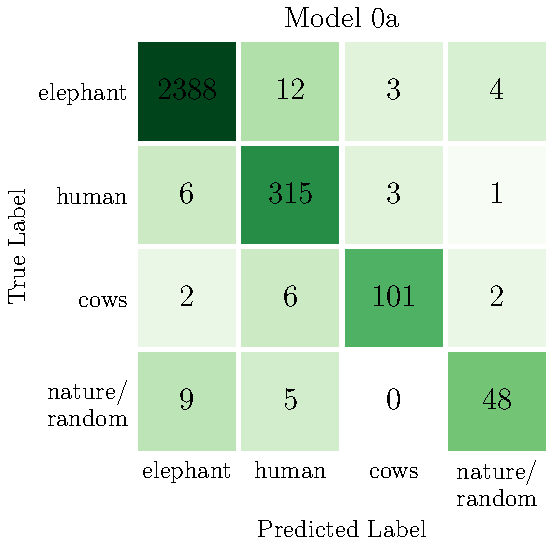
\includegraphics[width=1\linewidth]{0a_cm.pdf} 
    \end{subfigure}
    \begin{subfigure}{0.5\textwidth}
        \centering
        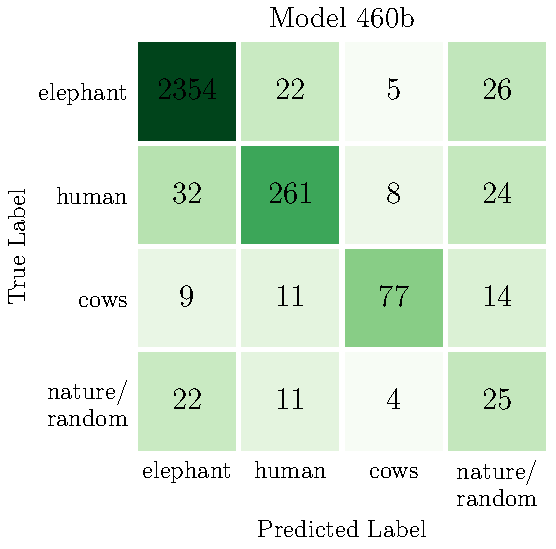
\includegraphics[width=1\linewidth]{460b_cm.pdf}
    \end{subfigure}
    \caption{Confusion matrices of \textit{0a} model (left) and \textit{460b} model (right).}
    \label{double_cm}
\end{figure}

\subsection{ Comparison of Edge Impulse models}

We wanted to take our 6 models and compare them against 6 Edge Impulse models that were created by using the same hyperparameters.
However, at the time of writing, Edge Impulse supported only model training on images of the same dimensions.
Images with different dimensions could either be cropped or scaled to fit a 1:1 ratio.
Using the same hyperparameters in Edge Impulse Studio that were used in our models, would always create a model with a smaller number of parameters.
The smaller image creates a smaller network when compared to a bigger image, given that the rest of the architecture does not change.
That meant that we could not make a direct comparison between our models and models trained in the Edge Impulse Studio.
We also could not perform a random search of hyperparameters in the Edge Impulse Studio, as this feature was not fully supported at the time of writing this thesis.

We decided to train a few differently sized models, using the same general CNN architecture as before, but with some minor changes in hyperparameter values.
We also trained a few models with the Transfer Learning technique.
Edge Impulse offers scaled-down versions of pre-trained MobileNetV2\footnotemark NN architecture, which we used.

Tables \ref{ei_models1} and \ref{ei_models2} show the properties of Edge Impulse models using CNN architecture and the Transfer Learning technique, respectively. 
Table \ref{precision_recall_table_ei} shows the calculated precision and recall values of Edge Impulse models using both approaches.
\footnotetext{MobileNetV2 is a efficient, lightweight NN architecture, designed for image recognition tasks, suitable for mobile applications\cite{geron}. MobileNetV2 contains a width multiplier hyperparameter, which scales up or down the total number of parameters, thus providing a trade-off between accuracy and computation complexity. Edge Impulse offers three different width multiplier options: 0.35, 0.1 and 0.05.}

We used only two different versions of MobileNetV2, 0.35, and 0.1, as we saw an accuracy drop in the reduction of the width multiplier hyperparameter.
In all cases the pre-trained model was followed by one or two dense layers, with dropout layers in between.
\newline
\begin{table}[!htbp]
    \centering
    \caption{ Properties of Edge Impulse models using the CNN architecture.}
    \rowcolors{2}{gray!25}{white}
    \makebox[\textwidth]{%
    \begin{tabular}{llllllllrl}
    \textbf{Model ID} & \rot{FilterNum1} & \rot{FilterNum2} & \rot{FilterNum3} & \rot{DenseSize} & \rot{DropoutRate}  &\rot{FilterSize} & \rot{LearningRate} & \rotatebox{45}{\parbox{2cm}{Number of parameters}} & \rot{Accuracy[\%]}  \\\toprule
        0ei & 72 & 80 & 64 & 72 & 0.4  & 3x4 & 0.0003 & 1,168,804 & 97.7\\
        1ei & 40 & 48 & 32 & 64 & 0.35 & 3x4 & 0.0001 &   503,196 & 97.5\\
        2ei & 40 & 20 & 20 & 48 & 0.25 & 3x4 & 0.0001 &   231,204 & 97.3\\
        3ei & 42 & 44 &  8 & 14 & 0.1  & 3x4 & 0.0003 &    52,272 & 96.6\\\bottomrule
    \end{tabular}}
    \label{ei_models1}
\end{table}
\clearpage
\begin{table}[!htbp]
    \centering
    \caption{ Properties of Edge Impulse models using the Transfer Learning technique.}
    \rowcolors{2}{gray!25}{white}
    \makebox[\textwidth]{%
    \begin{tabular}{llllllll}
        \textbf{Model ID} & \rotatebox{45}{\parbox{1cm}{Width \\Multiplier}} & \rot{DenseSize1} & \rot{DenseSize2} & \rot{DropoutRate} & \rot{LearningRate} & \rotatebox{45}{\parbox{2cm}{Number of\\parameters}} & \rot{Accuracy[\%]}  \\\toprule
        0tl & 0.35 & 16 & N/A& 0.1 & 0.0005 & 430,676 & 98.5\\
        1tl & 0.35 & 16 & 16 & 0.1 & 0.0005 & 430,948 & 98.4\\
        2tl & 0.35 & 32 & 32 & 0.1 & 0.0005 & 452,484 & 98.7\\
        3tl & 0.1  & 32 & 32 & 0.1 & 0.0005 & 135,732 & 95.7\\\bottomrule
    \end{tabular}}
    \label{ei_models2}
\end{table}
\begin{table}[!htbp]
    \caption{ Precision and recall metrics of trained Edge Impulse models}
    \rowcolors{2}{gray!25}{white}
    \makebox[\textwidth]{%
    \begin{tabular}{lrrrrrrrr}\toprule
        \textbf{Model ID}               & 0e    & 1e & 2e & 3e & 0tl & 1tl & 2tl & 3tl\\\toprule
        \textbf{Metrics}                &&&&&&&&\\\toprule
        Accuracy[\%]                    & \cellcolor{tbyellow} 97.7  
                                        & \cellcolor{tbyellow} 97.5  
                                        & \cellcolor{tbyellow} 97.3  
                                        & \cellcolor{tbyellow} 96.6  
                                        & \cellcolor{tbgreeny} 98.5  
                                        & \cellcolor{tbgreeny} 98.4  
                                        & \cellcolor{tbgreen} 98.7  
                                        & \cellcolor{tbred} 95.7  \\
        Number of parameters            & \cellcolor{tbred} 1,169K 
                                        & \cellcolor{tbyellow} 503K 
                                        & \cellcolor{tbgreeny} 231K 
                                        & \cellcolor{tbgreen} 52K 
                                        & \cellcolor{tbyellow} 430K 
                                        & \cellcolor{tbyellow} 431K 
                                        & \cellcolor{tbyellow} 452K 
                                        & \cellcolor{tbgreeny} 136K\\\midrule
        P of elephant class[\%]         & \cellcolor{tbgreen}  99.69 
                                        & \cellcolor{tbgreeny} 99.53 
                                        & \cellcolor{tbgreeny} 99.42 
                                        & \cellcolor{tbyellow} 99.27 
                                        & \cellcolor{tbyellow} 99.27 
                                        & \cellcolor{tbgreeny} 99.42 
                                        & \cellcolor{tbgreeny} 99.48
                                        & \cellcolor{tbred}    98.65 \\
        P of human class[\%]            & \cellcolor{tbyellow} 95.05 
                                        & \cellcolor{tbyellow} 95.05 
                                        & \cellcolor{tbyellow} 91.87 
                                        & \cellcolor{tbyellow} 91.52 
                                        & \cellcolor{tbgreen}  97.17 
                                        & \cellcolor{tbyellow} 95.41 
                                        & \cellcolor{tbgreeny} 96.47
                                        & \cellcolor{tbred}    85.16 \\
        P of cow class[\%]              & \cellcolor{tbyellow} 82.22 
                                        & \cellcolor{tbyellow} 78.89 
                                        & \cellcolor{tbyellow} 82.22 
                                        & \cellcolor{tbyellow} 79.57 
                                        & \cellcolor{tbgreen}  92.22 
                                        & \cellcolor{tbgreeny} 91.01 
                                        & \cellcolor{tbgreen}  92.22 
                                        & \cellcolor{tbred}    75.56 \\
        P of nature/random class[\%]    & \cellcolor{tbyellow} 63.04 
                                        & \cellcolor{tbyellow} 65.22 
                                        & \cellcolor{tbyellow} 73.91 
                                        & \cellcolor{tbred}    50.0  
                                        & \cellcolor{tbgreeny} 86.96 
                                        & \cellcolor{tbgreeny} 89.13 
                                        & \cellcolor{tbgreen}  91.3 
                                        & \cellcolor{tbyellow} 78.85 \\\midrule
        R of elephant class[\%]         & \cellcolor{tbgreen}  99.86 
                                        & \cellcolor{tbyellow} 98.91 
                                        & \cellcolor{tbyellow} 98.44 
                                        & \cellcolor{tbyellow} 98.65 
                                        & \cellcolor{tbgreeny} 99.48 
                                        & \cellcolor{tbgreeny} 99.27 
                                        & \cellcolor{tbgreeny} 99.37 
                                        & \cellcolor{tbred}    98.03 \\
        R of human class[\%]            & \cellcolor{tbyellow} 93.4  
                                        & \cellcolor{tbyellow} 92.44 
                                        & \cellcolor{tbgreeny} 94.2  
                                        & \cellcolor{tbred}    88.4  
                                        & \cellcolor{tbgreeny} 94.5  
                                        & \cellcolor{tbgreen}  95.74 
                                        & \cellcolor{tbgreen}  95.79 
                                        & \cellcolor{tbyellow} 90.26 \\
        R of cow class[\%]              & \cellcolor{tbyellow} 90.24 
                                        & \cellcolor{tbyellow} 86.59 
                                        & \cellcolor{tbyellow} 84.09 
                                        & \cellcolor{tbyellow} 79.57 
                                        & \cellcolor{tbgreeny} 92.22 
                                        & \cellcolor{tbyellow} 89.01 
                                        & \cellcolor{tbgreen} 94.32 
                                        & \cellcolor{tbred} 67.33 \\
        R of nature/random class[\%]    & \cellcolor{tbyellow} 87.88 
                                        & \cellcolor{tbyellow} 88.24 
                                        & \cellcolor{tbyellow} 94.44 
                                        & \cellcolor{tbgreeny} 95.83 
                                        & \cellcolor{tbgreeny} 95.24 
                                        & \cellcolor{tbgreen} 97.62 
                                        & \cellcolor{tbgreeny} 95.45 
                                        & \cellcolor{tbyellow} 91.11 \\\bottomrule
    \end{tabular}}
    \label{precision_recall_table_ei}
\end{table}

Some observations:
\begin{itemize}
    \item Models using CNN architecture did not out perform our models in terms of accuracy. Models \textit{2a} and \textit{0b} both had accuracy of 98.04 \%, while none of the Edge Impulse models with CNN architecture passed 98 \%.
    \item Most of the models trained with the Transfer Learning technique outperformed our models.
    \item Model \textit{2tl} performed exceptionally well, reaching an accuracy of 98.7 \% while having a relatively small number of parameters.
    \item We saw that by decreasing the width multiplier, we did not benefit much in accuracy as much as we lost in model size. Even increasing the sizes of dense layers did not solve the problem. 
\end{itemize}


\section{ On-device performance testing}

Performance testing of all models was done on an STM32F767ZI microcontroller, running at 216 \si{\mega\hertz}.
Testing of our models was done by using the MicroML framework that we wrote, which called TFLite Micro API directly.
Testing of Edge Impulse models was done on Mbed OS, as this platform is supported by Edge Impulse, and they already provide an example for it.
We could not test model \textit{0a} on the device as the TFLite converter failed to produce a compilable model.

To time the execution of our code we used Data Watchpoint Trigger (DWT) which contains a counter that is incremented directly by the system clock.
DWT does not use interrupts, therefore it does not introduce the overhead of calling interrupt routines as systick timer does.


Edge Impulse provides examples for testing out of the box, so not much work is needed to get the first-order approximation of performance.
For profiling, the code execution Mbed API was used, which uses timer interrupts to track elapsed time.
Figure \ref{speed_comp} shows models ranked from the fastest to the slowest with marked corresponding accuracies and inference times.

\begin{figure}[ht]
    \centering
    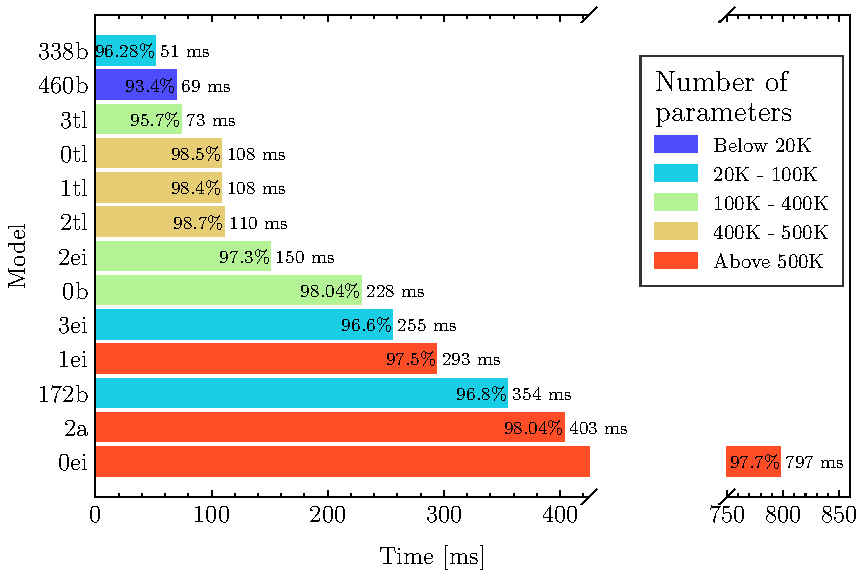
\includegraphics[width=1\linewidth]{speed_comp.pdf}
    \caption{ Comparison of time of inference of different models.}
    \label{speed_comp}
\end{figure}

We can see that all models performed inference in less than 1 second, which was a constraint that we set earlier in Section \ref{model_obj}.
The best time wise performing model was \textit{338b}, with an inference time of 51 \si{\milli\second}, but there are also many models that perform inference in under 300 \si{\milli\second}.

We also discovered some unexpected trend in the results.
We assumed that inference time is proportional to the number of parameters if the general structure of the model remains the same.
As can be seen in Figure \ref{speed_comp}, there are few exceptions to this rule; model \textit{338b} executed inference faster than \textit{460b}, although it has more parameters (20K versus 13K).
Model \textit{172b} was slower than \textit{0b}, although it has five times less parameters.
This behaviour is not exclusive only to our models, but it can be seen in Edge Impulse models as well, for example, models \textit{2ei} and \textit{1ei}.

Edge Impulse models trained with the Transfer Learning technique \textit{0tl}, \textit{1tl}, \textit{2tl} and \textit{3tl} should not be compared to other models in this sense, as the architecture of MobileNetV2 contains additional different operations.

We can only speculate about the reason for this behaviour, since it is present both in our models and Edge Impulse models, and we can assume this to be a TFLite bug.

\subsection{ Comparison of code sizes}

We also wanted to inspect the Flash and RAM sizes of binaries that we compiled for on-device testing.
For this task we used the \verb|arm-none-eabi-size| command line tool, which returns sizes of \verb|text|, \verb|data|, \verb|bss| sections in bytes, and an example of its output can be seen in Figure \ref{size_output}.
To compute the used Flash we simply had add bytes from \verb|text| and \verb|data| sections, and to compute used RAM we added together \verb|data| and \verb|bss| sections\footnotemark.
\footnotetext{ A data section which contains initialised static variables is first placed into Flash memory and is copied to RAM before the program enters the main function. That is why we have to account for an additional \verb|data| section in Flash memory.}
\lstset{style=mystyle}
\begin{figure}[ht] 
\begin{lstlisting}[language=bash]
$ arm-none-eabi-size firmware.elf
   text	   data	    bss	    dec	    hex	filename
 149124	    388	  47064	 196576	  2ffe0	firmware.elf
\end{lstlisting}
\captionof{lstlisting}{ Example output of arm-none-eabi-size command.}
\label{size_output}
\end{figure}
\newline
Code sizes for all models are presented in Figure \ref{size_comp}, models are ordered the same way as they have been in Figure \ref{speed_comp}.
\begin{figure}[ht]
    \centering
    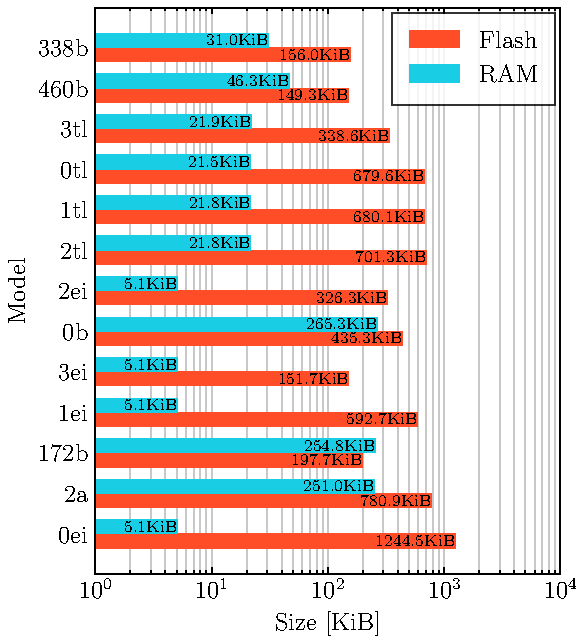
\includegraphics[width=1\linewidth]{size_comp.pdf}
    \caption{ Comparison of Flash and RAM size of compiled example models.}
    \label{size_comp}
\end{figure}

We can see that all of our models generally use more RAM then Edge Impulse models.
This is due to how the inference is executed.
TFLite Micro uses a generic interpreter approach, where the model is loaded at runtime.
Edge Impulse uses a compiled approach, which they named The EON\textsuperscript{TM} Compiler\cite{eon}.
The EON\textsuperscript{TM} Compiler still uses TFLite Micro, however, it does not use its interpreter, but calls operation kernels directly.
This means that the linker knows exactly which operations are used and more data can be moved into Flash, thus eliminating unneeded code size\cite{eon}.


\subsection{ Comparison of different optimisations}

Some extra amount of work and research was required to be able to run the ML inference at maximum possible efficiency under MicroML.
Figure \ref{opt_comp} shows the reductions in inference time of the \textit{0b} model while using different optimisation methods.
\newline

\begin{figure}[ht]
    \centering
    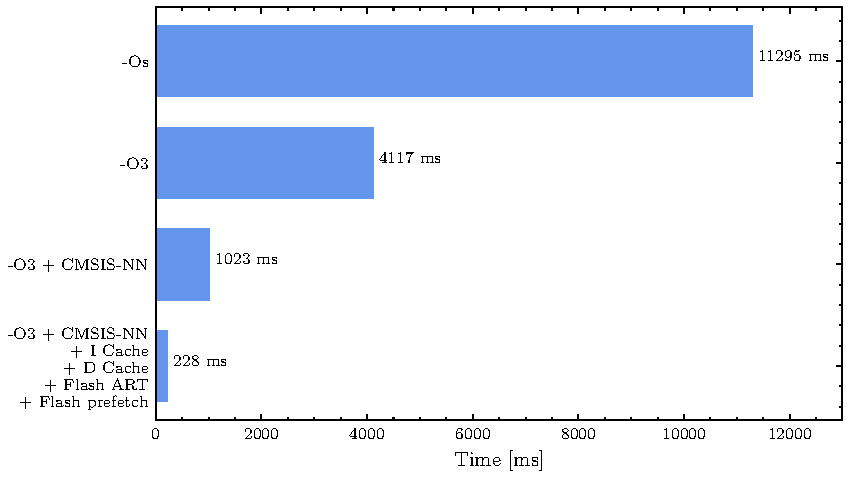
\includegraphics[width=1\linewidth]{opt_comp.pdf}
    \caption{ Inference time of the \textit{0b} model using different optimisations.}
    \label{opt_comp}
\end{figure}

We started with no optimisations at all, while using only the \verb|-Os| compiler flag.
The \verb|-Os| flag generally optimises for minimal size, it enables all \verb|-O2| optimisations, except those that increase in size.
This optimisation level is often used, however, we found out that the inference time of more than 11 seconds was too long.

Changing optimisation level to \verb|-O3| decreased the time of inference drastically, down to 4117 \si{\milli\second}.
\verb|-O3| turns on all \verb|-O2| optimisations plus additional ones, and disregards any code size optimisations completely.

Changing compiler optimisation flags could not lower the time of inference any further, so other approaches were needed.
While reading through the TensorFlow documentation we saw that it supports the CMSIS-NN library for ARM microcontrollers.
CMSIS-NN is a collection of efficient Neural Network kernels, that intends to maximise performance and lower code size of NN models implemented on ARM microcontrollers.
TensorFlow provides wrappers for some of these kernels, such as convolutional, fully connected, pooling layers and others.
Not much work was needed to use these highly efficient kernels, as we only needed to specify in our Makefile that we wanted to compile CMSIS-NN kernels and not compile generic TensorFlow kernels. 
Time of inference dropped by about 3 seconds, down to 1023 \si{\milli\second}.

As we saw that similarly sized Edge Impulse models were running much faster on the Mbed platform compared to our MicroML code while using the same microcontroller, we knew that there was another step left.
The final performance increase was reached by using features only fully found in Cortex-M7 microcontrollers and partly in Cortex M3/4 microcontrollers. 
To achieve it we had to enable I and D caches, flash prefetch and flash ART.

ART stands for Adaptive Real-Time memory accelerator, which encompasses I/D caches and a flash prefetch buffer.
I and D caches are small, efficient portions of memory, which are located in the CPU of the microcontroller.
They hold instructions and data respectively, and if those are requested by the next microcontroller instruction, they can be read much faster compared to reading them from flash memory. 
By enabling flash prefetch the microcontroller reads additional sequential instructions into the prefetch buffer, thus enabling execution without any wait states (if the instruction flow is sequential).
Elimination of wait states improved the time of inference greatly, as it was decreased to 228 \si{\milli\second}.


\subsection{ Scoring trained models}\label{scoring_models}

Choosing the best model for on-field deployment is a hard task due to many different metrics: Precision and recall values, time of inference, and code size.
To make this job easier we devised a scoring system: Each metric was going to be normalised and multiplied with some weight value.
All products would then be summed up, and the result would represent the final score.
The sum of the weights was equal to 100, which means that the possible maximum score was also 100.
We decided to allocate 50 weight points to all precision and recall values, 30 points to the time of inference value, 5 points for Flash size and 15 points for RAM size.
As we cared more about the precision and recall values of the elephant, human and cow classes, we gave them 7 weight points each, while the nature/random class received only 4.
We valued Flash size less than RAM, as most of the microcontrollers have much less RAM than they do Flash, thus, we gave 15 weight points to RAM size and only 5 to Flash size.

Since the time of inference, Flash and RAM sizes are properties which should give a larger score, the smaller they were, we mapped them into a range between 0 and 1.
The smallest value inside the set would be assigned 1, the biggest 0, the values in between were mapped linearly.

Scoring is described mathematically in \ref{score_equ}, while the final results can be seen in Figure \ref{score_comp}.
\begin{equation}\label{score_equ}
    \begin{aligned}
        Score[i] ={} & 7 K(P_{elephant},i) + 7 K(P_{human},i) + 7 K(P_{human},i) + 4 K(P_{ntr/rnd},i) \\
                     & +{} 7 K(R_{elephant},i) + 7 K(R_{human},i) + 7 K(R_{human},i) + 4 K(R_{ntr/rnd},i) \\
                  & +{} 30\: F(ToI, i) +5\: F(Flash, i) + 15\: F(RAM, i)   \\
                  & \\
        K(X, i) ={}  & \frac{(X[i] - MIN(X))}{MAX(X)- MIN(X)} \\
                  & \\
        F(X, i) ={}  & \frac{(X[i] - MAX(X))}{MIN(X)- MAX(X)}
    \end{aligned}
\end{equation}
Where:\\
$Score$ - Vector of calculated scores\\
$i$ - i$^{th}$ model\\
$P_{j}$ - Vector of precision values of the j$^{th}$ class\\
$R_{j}$ - Vector of recall values of the j$^{th}$ class\\
$ToI$ - Vector of Time of Inference values\\
$Flash$ - Vector of Flash sizes\\
$RAM$ - Vector of RAM sizes\\
$K(X,i)$ - Normalising function with vector X and element index i as arguments\\
$F(X,i)$ - Normalising, inverting, function with vector X and element index i as arguments\\
$MAX(X)$ - Function that finds the maximum element in vector X\\
$MIN(X)$ - Function that finds the minimum element in vector X
\begin{figure}[ht]
    \centering
    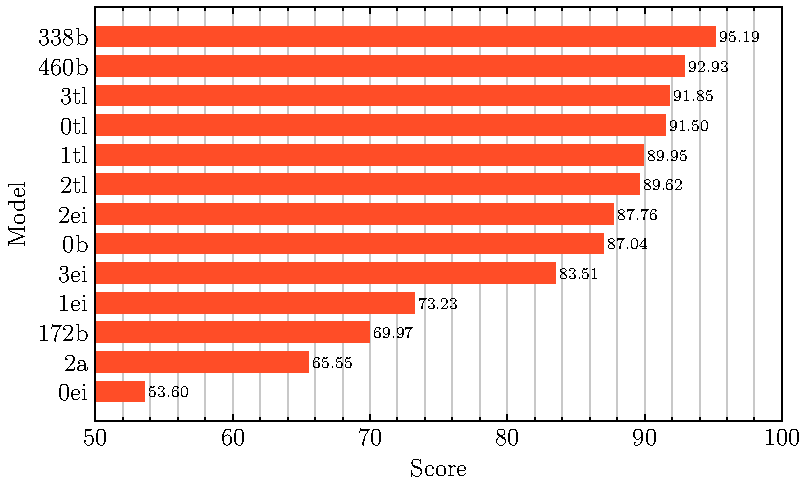
\includegraphics[width=1\linewidth]{score_comp.pdf}
    \caption{ Score comparison of different models}
    \label{score_comp}
\end{figure}

\section{ Summary of model testing}

As we saw in Figure \ref{score_comp} model \textit{3tl} received the highest score, and models \textit{1tl}, \textit{2tl} followed.
This should not be a surprise, because models trained with Transfer Learning achieved high accuracies and executed inference in about 100 \si{\milli\second}. 
Additionally, the compiled approach for computing Neural Networks keeps the used Flash and RAM sizes to a minimum.
We saw that using a number of different optimisations was critical to achieving low inference times, thus making ML on the embedded device viable.

\section{ Power profiling of an embedded early warning system}

\subsection{ Measuring setup}

To measure power consumption we used a product called Otii Arc (Otii), which can be seen in Figure \ref{otii}.
Otii, made by the company Qoitech, is a small portable box, that contains a power supply, a current and voltage measurement unit and a data acquisition module.
It connects to a computer over a USB cable, and can be powered through it or with an external charger.

It can provide output voltage between 0.5 V and 4.55 V, and has accuracy of $\pm$(0.1 \% + 50 nA) when measuring current.
It is a perfect tool for evaluating low-power systems.
\newline
\begin{figure}[ht]
    \centering
    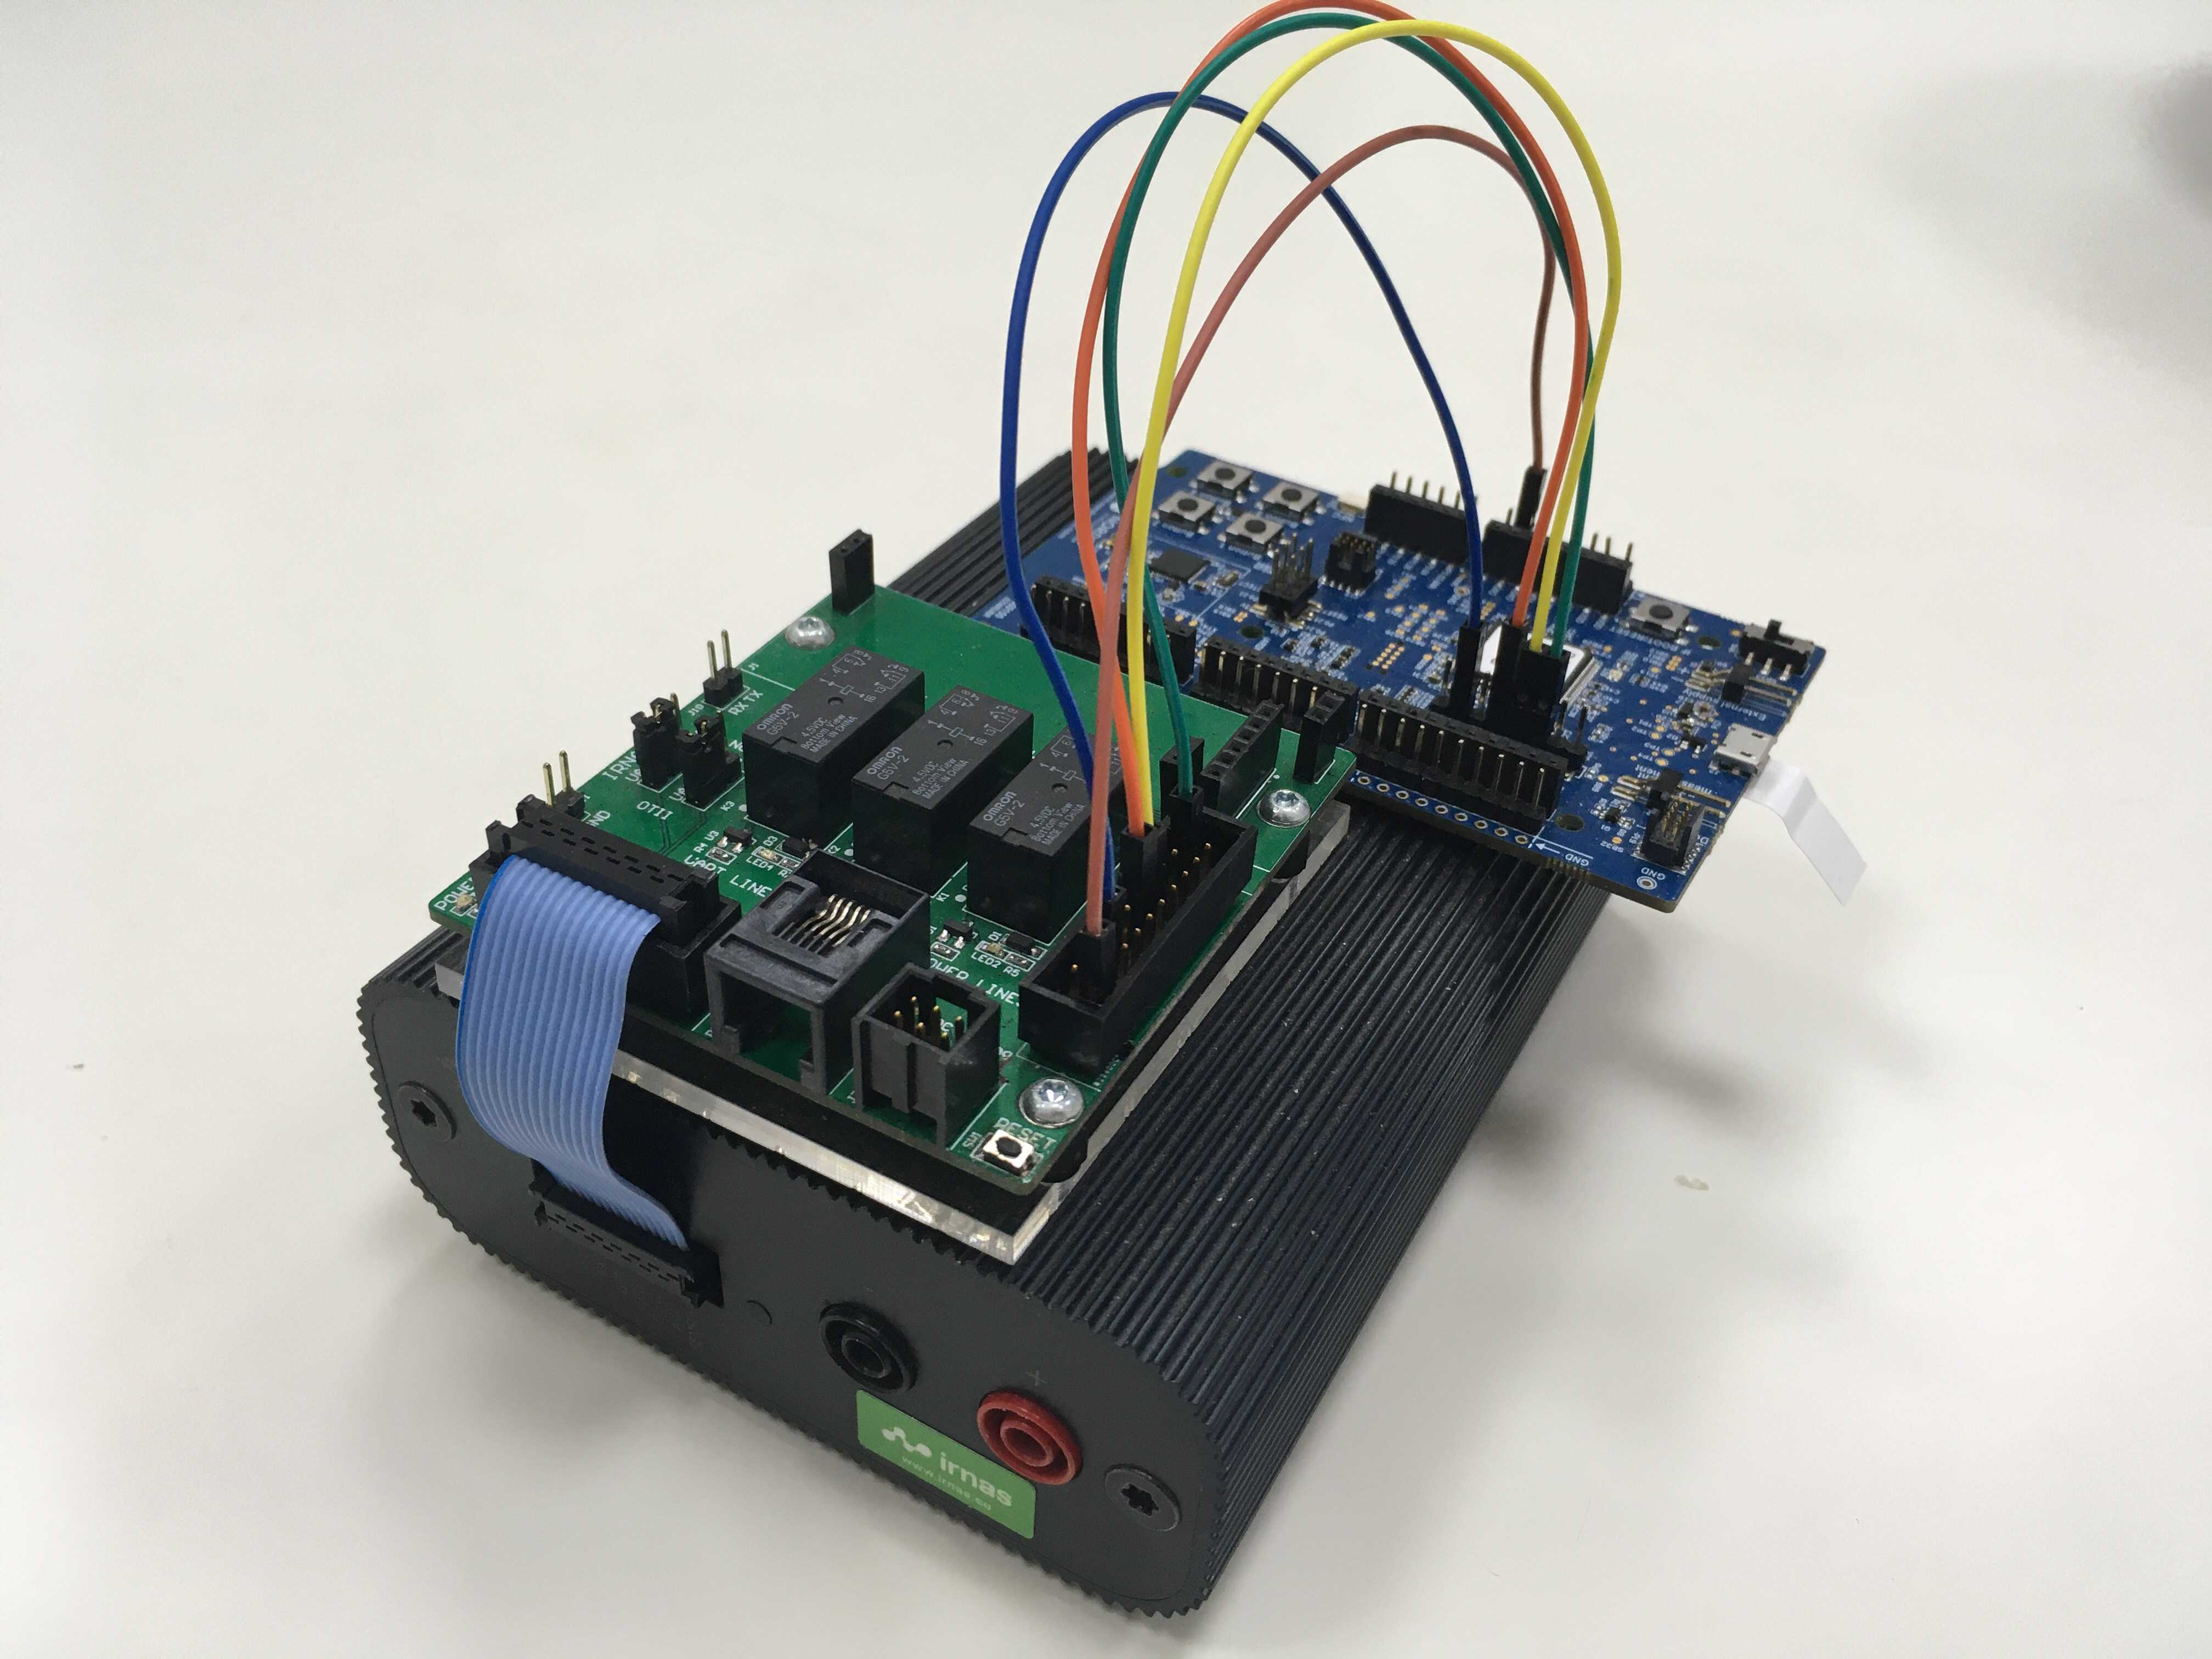
\includegraphics[width=0.75\linewidth]{otii.jpg}
    \caption{ Otii Arc with nRF52832 DK and added measurement board made by IRNAS.}
    \label{otii}
\end{figure}

Measurements analysis is done with a desktop application, example of it is seen in Figure \ref{otii_screen}. 
The application enables users to select a part of the measurement, for which it computes minimum, maximum and average values automatically.
To present our results we exported the current measurements in CVS format and plotted them with Matplotlib.

In the following Section we evaluated the power consumption of our embedded early warning system.
We first measured the power consumption of the nRF52 microcontroller in a low-power state, then we connected the LR1110 evaluation shield to the nRF52840 DK board and repeated the measurement.
We then connected Nucelo-F767ZI and the FLIR camera, and measured power consumption of the whole detection sequence.
\begin{figure}[ht]
    \centering
    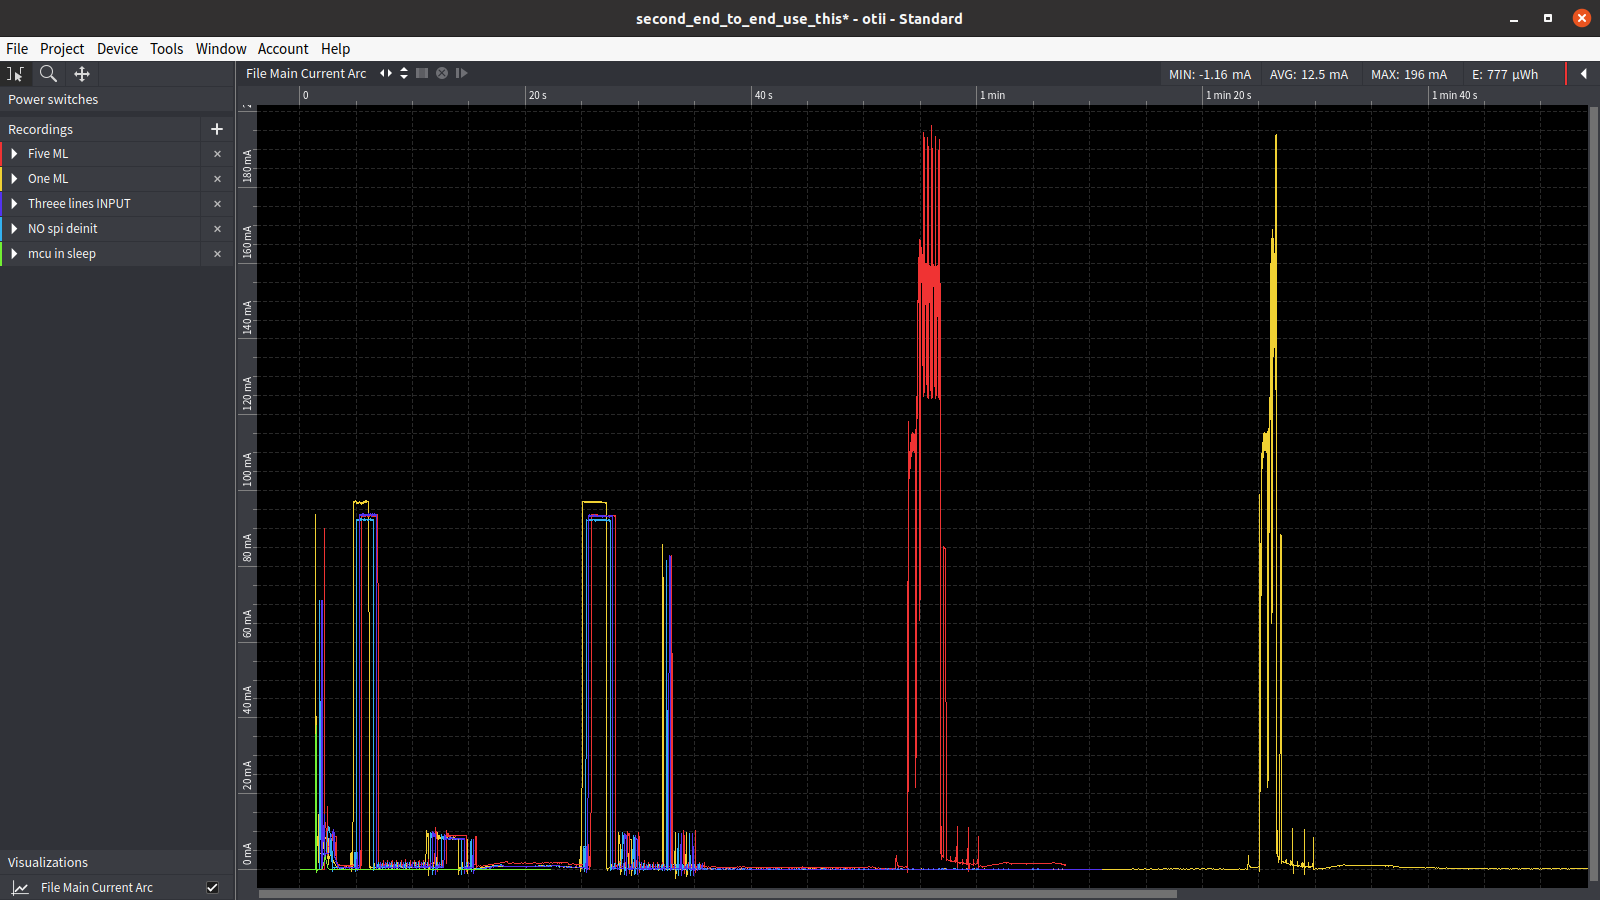
\includegraphics[width=1\linewidth]{otii_screenshot.png}
    \caption{ Screenshot of Otii user interface.}
    \label{otii_screen}
\end{figure}

\subsection{ Current measurements}

We conducted all our measurements with Otii's output voltage set to 3.3 V.
Before measuring the current consumption of the whole image processing sequence we wanted to evaluate the current consumption of the nRF52 microcontroller in the low-power state.
In a Zephyr kernel such procedure is relatively simple; type of sleep mode is configured with a Kconfig file and the microcontroller transitions into it whenever it enters the lowest idle thread.
Peripherals require special attention, as it needs to be specified explicitly which one needs to be turned off.
We turned off both of the UART peripherals and the SPI peripheral, while keeping GPIO active, as we needed a GPIO interrupt to wake nRF52 up from a low-power state.
We also had to make sure that the nRF52 microcontroller was completely disconnected from the on board J-Link debug probe to avoid any unnecessary current leaks.
Luckily, the nRF52840 development board has an analogue switch, which does exactly that.
To measure current consumption we simply connected the voltage output of Otii to the external power pins of the nRF52840 DK board.
Figure \ref{mcu_in_sleep} shows the current consumption in the low-power state.
\newline
\begin{figure}[ht]
    \centering
    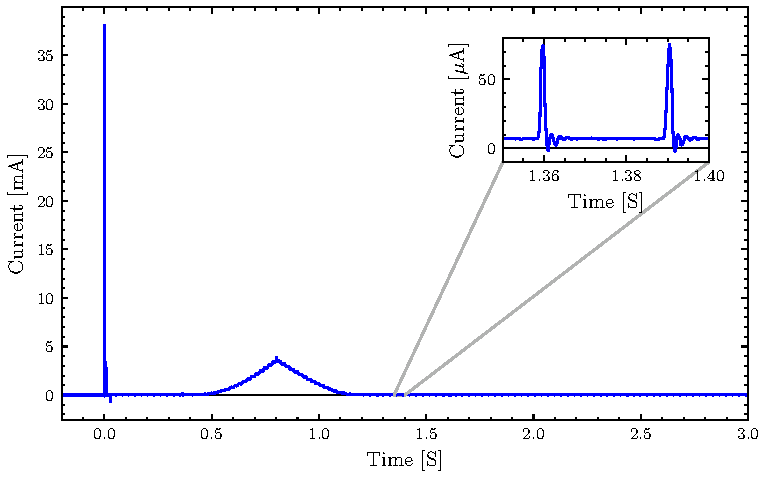
\includegraphics[width=1\linewidth]{mcu_in_sleep.pdf}
    \caption{ Current consumption of nRF52840 microcontroller in low-power state.}
    \label{mcu_in_sleep}
\end{figure}

The initial spike at the beginning of the graph happens due to the many decoupling capacitors on the board.
Due to the sudden change in voltage their impedance is low, therefore, more current is drawn.
The pyramid looking shape between 0.5 and 1 second happens due to the onboard regulators turning on.

The smaller graph inside Figure \ref{mcu_in_sleep} shows a close up view of the current consumption.
The peaks reached 70.3 \si{\micro\ampere}, steady state was at 6.9 \si{\micro\ampere}, while the average current was 9.1 \si{\micro\ampere}.
Peaks were repeating at a frequency of 33.3 \si{\hertz}.
\clearpage
The measured average current was higher than expected, according to the nRF52's datasheet\cite{nrf52_datasheet} current consumption should be 3.16 \si{\micro\ampere}.

In the next measurement we connected the LR1110 shield to the nRF52840 DK board, and observed the current consumption of the initial LoRaWAN join sequence.
The current profile of it can be seen in Figure \ref{lora_join}.
\newline
\begin{figure}[ht]
    \centering
    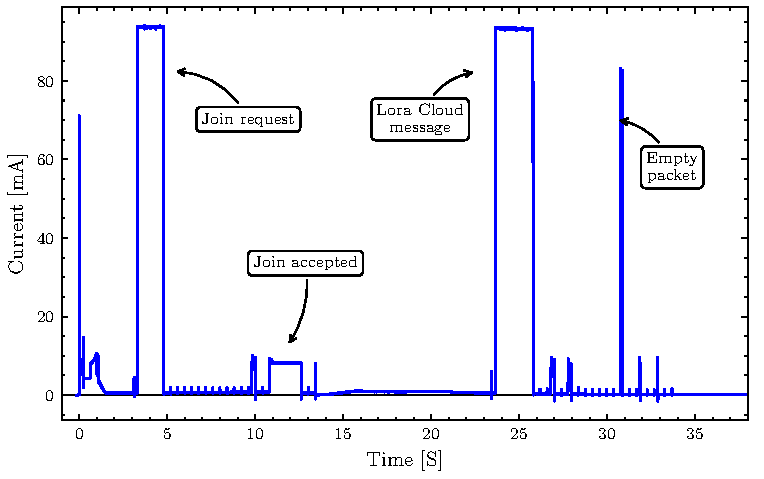
\includegraphics[width=1\linewidth]{lora_join.pdf}
    \caption{ Current profile of the LoRaWAN join sequence.}
    \label{lora_join}
\end{figure}

Besides the initial spike, we can see an additional four pulses afterwards, with some smaller spikes in between. 
As we are using Over-The-Air Activation (OTAA), the LR1110 first has to negotiate for a set of keys with the server before it can start transmitting.
This happens in first the two pulses; LR1110 first sends a join request and then listens for a response.
After receiving a response it confirms it.
In the third pulse LR1110 sends a message that is a part of the LoRa Cloud service.
This message is specific to LR1110, and it cannot be disabled completely.
The last, thin pulse belongs to an empty payload message, which LR1110 always transmits in the beginning.
The average current consumption of the LoRaWan join procedure is 11.4 \si{\milli\ampere} and lasts for about 34 seconds.
Average current consumption in sleep state increased to 76.8 \si{\micro\ampere}.

In our next test we connected the nRF52 to a boost converter circuit, Nucleo-F767ZI and FLIR Lepton camera, setup can be seen in Figure \ref{measure_setup}.
We did not use a PIR sensor as a wakeup source, as we saw that its detection was too sensitive to its surroundings and we could not control it completely.
Instead we used a button on the nRF52840 DK as a wakeup interrupt.
To account for PIR sensor current consumption in later calculations we measured it separately, and we saw that it drew 130 \si{\micro\ampere}.
\begin{figure}[ht]
    \centering
    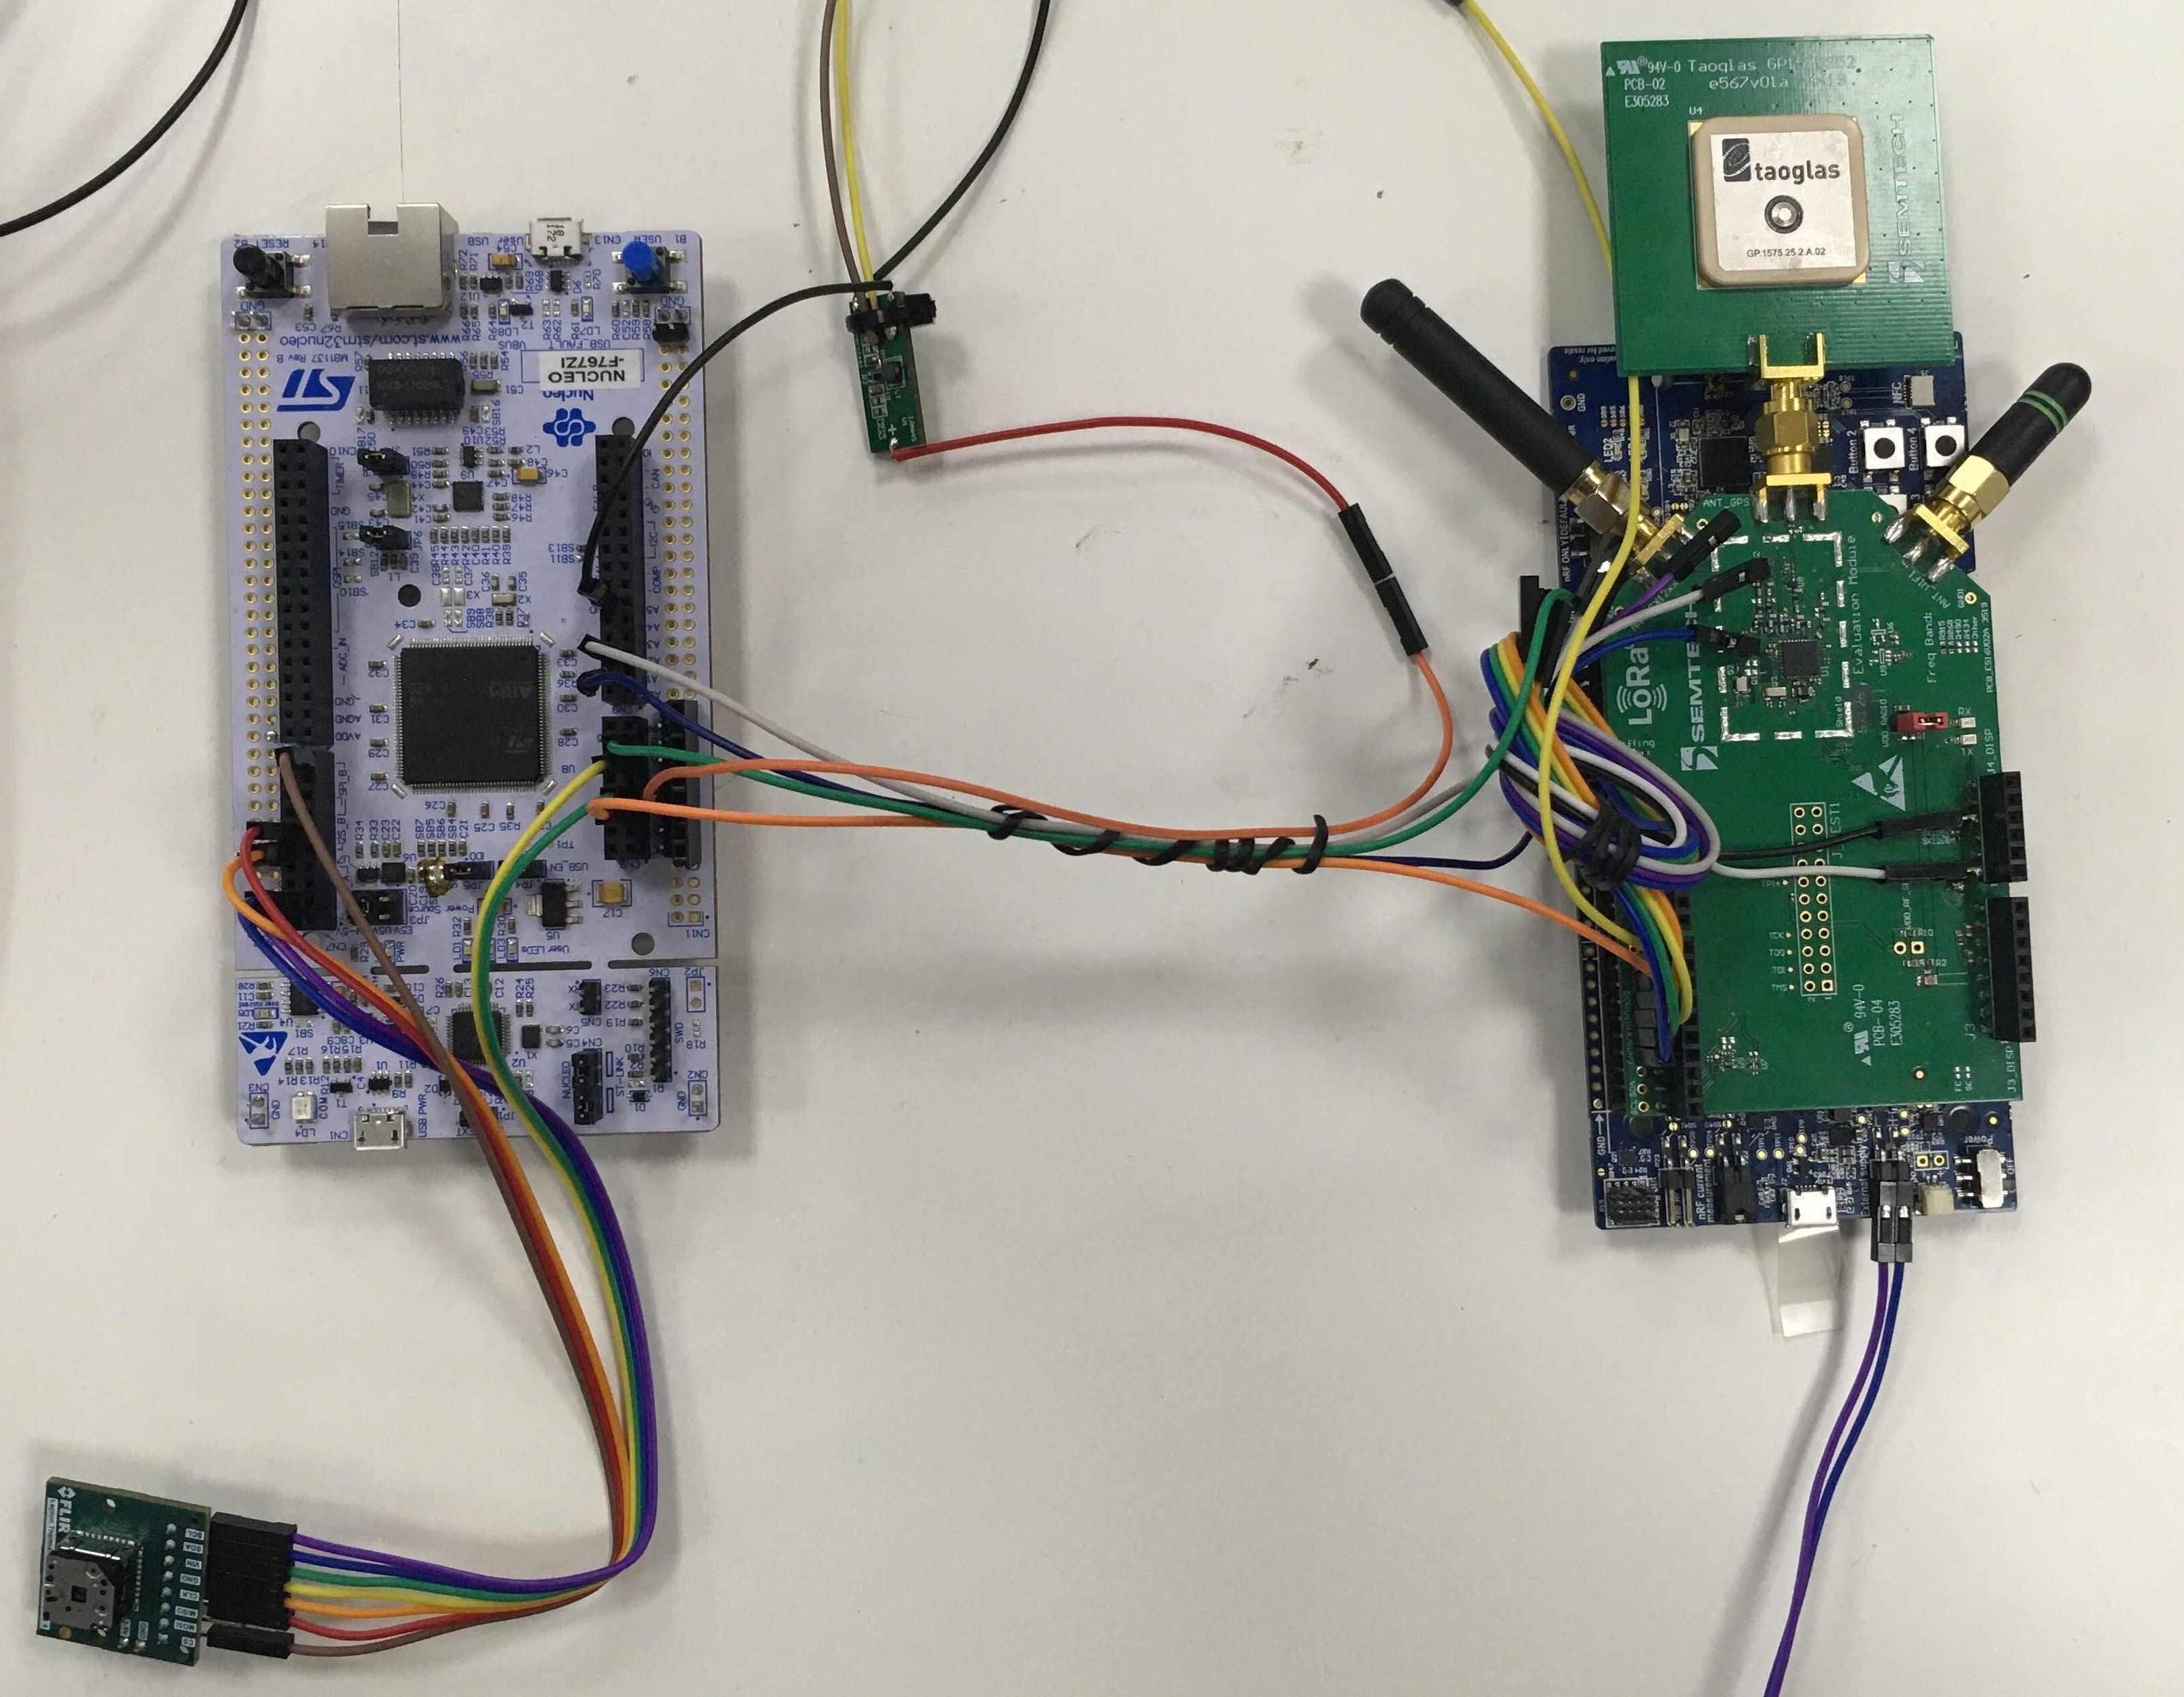
\includegraphics[width=0.75\linewidth]{measure_setup.jpg}
    \caption{ Device under test: nRF52840 DK with attached LR1110 shield, boost converter breakout board, Nucleo-F767ZI and FLIR Lepton camera.}
    \label{measure_setup}
\end{figure}

Since we wrote our firmware with libopencm3 in mind, we could not use the best performing model \textit{3tl}, as Edge Impulse models could only run on the Mbed platform.
We used our model \textit{460b} instead, as it was most similar to \textit{3tl} in terms of inference time (69 \si{\milli\second} compared to 73 \si{\milli\second}).
We captured two different inference procedures; in the first image capture and inference were done once, in the second one they were repeated 5 times.
Procedures can be seen on Figures \ref{one_ml} and \ref{five_ml} respectively.
Both procedures were followed by a LoRaWAN message that reported results to the server.

In the case where image capture and inferencing happened once, we measured the total time of the whole detection procedure to be about 1480 \si{\milli\second}, not including the time needed for the LoRaWAN message.
Average current consumption for this period was 114 \si{\milli\ampere}.
The measured average current of the whole event, shown in Figure \ref{one_ml} between 0 and 6 seconds, was 30 \si{\milli\ampere}.

In the case where image capture and inferencing happened five times, we measured the total time of the whole detection procedure to be about 2,960 \si{\milli\second}, not including the time needed for the LoRaWAN message.
Average current consumption for this period was 131 \si{\milli\ampere}.
If we add the transmission of the LoRaWAN message to the measured current consumption, thus increasing the time of the whole detection event to 8 seconds, we measure 51.9 \si{\milli\ampere}.

\begin{figure}[ht]
    \centering
    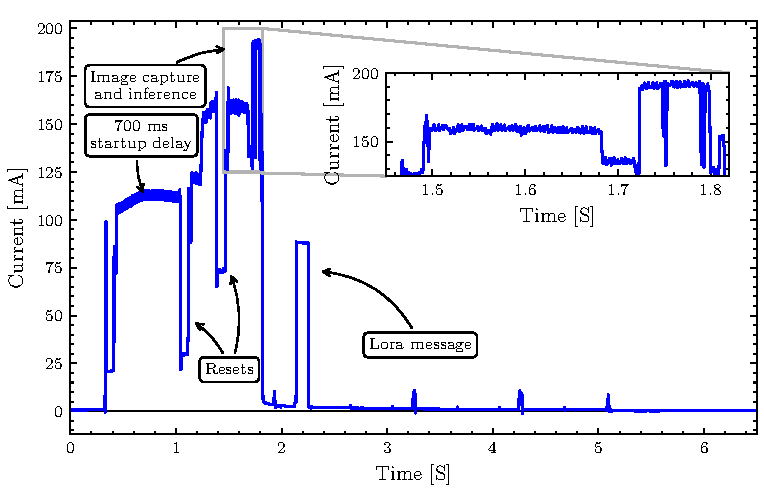
\includegraphics[width=1\linewidth]{one_ml.pdf}
    \caption{ Current profile of image capture and inference procedure.}
    \label{one_ml}
\end{figure}
\begin{figure}[ht]
    \centering
    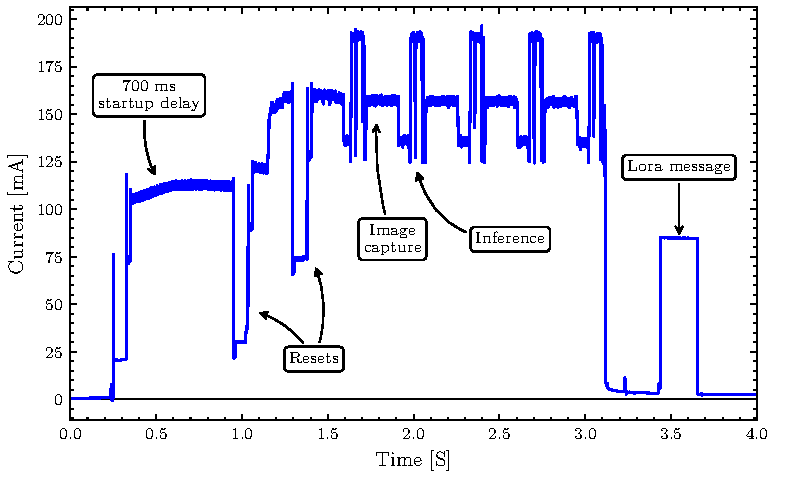
\includegraphics[width=1\linewidth]{five_ml.pdf}
    \caption{ Current profile of image capture and inference procedure repeated 5 times.}
    \label{five_ml}
\end{figure}

\subsection{ Commentary of the current measurement results}

The measured low-power state of nRF52, visible in Figure \ref{mcu_in_sleep}, was higher than expected.
nRF52's datasheet\cite{nrf52_datasheet} specifies current consumptions in many different conditions, which depend on: Type of sleep mode (System ON or System OFF, the latter loses execution context at wakeup), the amount of RAM retention and type of wakeup event.
Consumption can range from 0.95 \si{\micro\ampere} to 17.37 \si{\micro\ampere}.
Because Zephyr provides only abstract interface to power management, implementation of which is platform dependent, further research is needed to determine which exact nRF52 sleep mode Zephyr uses.
We assumed an expected current consumption of 3.16 \si{\micro\ampere} as this is the specified current consumption in System ON mode with full RAM retention and LFRC set as a wakeup event.
Another reason for increased power consumption could also be inadequate support circuitry of the nRF52840 DK board.

When we connected the LR1110 shield to the nRF52840 DK board we saw that average current consumption increased to 76.8 \si{\micro\ampere}, which was much more than expected.
LR1110 enters sleep mode automatically when it is finished with communication; according to its datasheet\cite{lr1110_datasheet}, current consumption should be around 1.85 \si{\micro\ampere}.
This current consumption is plausible, as we observed it in other IRNAS's products that use the LR1110 chip.
We suspect that the incorrect state of common GPIO connections between LR1110 and nRF52 was the reason for the increased current consumption, although, we were not able to fix the problem.

We mentioned that the time required for detection was about 1480\si{\milli\second}, if we captured one image and processed it or 2960 \si{\milli\second}, if done five times.
We can see that both detection procedures started with 700 \si{\milli\second} of delay.
According to the FLIR Lepton's datasheet \cite{flir_datasheet}, a delay is required before we can start communicating with the camera over the TWI interface.
Two microcontroller resets are visible, during our testing we saw that we could not communicate with the camera properly, if we did not reset the STM32 twice before that.
To accomplish this we simply connected the reset pin of STM32 with one of available nRF52 GPIO pins.


\subsection{ Battery life estimations}

Table \ref{lifetime_data} shows parameters values that we used in \ref{lifetime_equ} to calculate battery lifetime.
We defined a detection as a sequence where image capture and inference were repeated 5 times and then followed by a LoRaWAN message.
In our calculation we also accounted for one daily LoRaWAN message, which would report system status.
We assumed that the system is in low-power mode when it is not performing detection sequence or sending a LoRaWAN message.
As a power source we chose a lithium-ion cell battery NCR 18650B of the manufacturer Panasonic.
Its properties can be seen in Table \ref{lifetime_data}.

\begin{table}[ht]
    \centering
    \caption{ First hyperparameter search space}
    \rowcolors{2}{white}{gray!25}
    \begin{tabular}{lr}    \toprule
        \textbf{Event}                          & \textbf{Current consumption at 3.3 V} \\\midrule
        Low-power state                         & 76.8 \si{\micro\ampere}                \\ 
        PIR                                     & 130 \si{\micro\ampere}                 \\ 
        PIR and low-power state                 & 206.8 \si{\micro\ampere}               \\
        Detection sequence, 8 s                 & 51.9 \si{\milli\ampere}                \\
        LoRaWAN message, 230 \si{\milli\second} & 80 \si{\milli\ampere}                 \\\midrule
        \textbf{Battery type}                   & \textbf{Properties}                   \\
        Panasonic NCR 18650B                    & Nominal Voltage: 3.6 V                \\
                                                & Nominal Capacity: 3350 \si{\milli\ampere\hour}\\\bottomrule
    \end{tabular}
    \label{lifetime_data}
\end{table}

\begin{equation}\label{lifetime_equ}
\begin{aligned}
    P_{sleep} ={} & U_{supplied}\; I_{sleep}\\
P_{detect} ={} & U_{supplied}\; I_{detec}\\
P_{lora} ={} & U_{supplied}\; I_{lora}\\
t_{sleep}     ={} & 24h - t_{detect}\; N_{detect} - t_{lora}\\
P_{average}   ={} & \frac{P_{sleep}\; t_{sleep} + P_{detect}\;t_{detect}\; N_{detect} + P_{lora}\; t_{lora}}{24h}\\
t_{lifetime}  ={} & \frac{U_{bat}\;Ah_{bat}\;N_{bat}}{P_{average}}
\end{aligned}
\end{equation}

Where:\\
$U_{supplied}$ - Voltage at which we did our measurements, 3.3 V\\
$U_{bat}$ - Battery nominal voltage, 3.6 V\\
$Ah_{bat}$ - Battery nominal capacity, 3350 \si{\milli\ampere\hour}\\
$I_{lora}$ - Current consumption when sending a LoRaWAN message\\
$I_{sleep}$ - Current consumption of low-power state with PIR consumption\\
$I_{detect}$ - Current consumption of detection sequence\\
$P_{sleep}$ - Used power of low-power state and PIR\\
$P_{detect}$ - Used power of detection sequence\\
$P_{lora}$ - Used power of LoRaWAN message send\\
$P_{average}$ - Average power needed for the system to operate\\
$t_{detect}$ - Time spent in detection sequence in hours\\
$t_{sleep}$ - Time spent in low-power state in hours\\
$t_{lora}$  - Time spent sending LoRaWAN messages\\
$t_{lifetime}$ - Battery life time in hours\\
$N_{detec}$ - Number of detections in a day\\
$N_{bat}$ - Number of batteries

Because we could only assume how frequently our system had to perform the detection sequence, we repeated our calculation for several different numbers of detections per day.
We also varied the number of battery cells.
The enclosure that we planned to use had enough space for up to 6 battery cells.
The results of the estimations can be seen in Figure \ref{lifetime_figure}.
The X axis represents the number of battery cells, the Y axis represents the system life time in months, and the colour of the lines represents the number of detections per day, from 100 to 600.

\begin{figure}[ht]
    \centering
    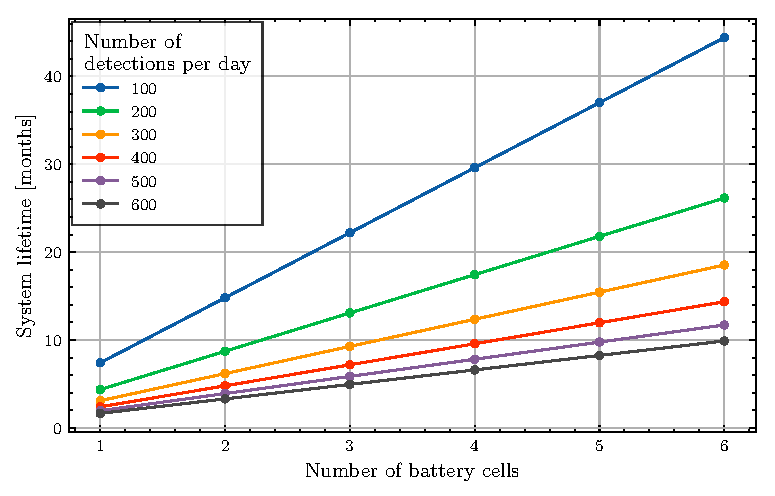
\includegraphics[width=1\linewidth]{lifetime.pdf}
    \caption{ Current profile of image capture and inference procedure.}
    \label{lifetime_figure}
\end{figure}

Results were promising, we can see that most battery configurations lasted more than 6 months, which is a long time, considering the application.
If we decide on a 6 battery cell configuration, we see that in the worst case where we are executing 600 detections per day, we can expect a system lifetime of 10 months, which is more than enough.
There are some things that we have to take into account.
We assumed 100 \% battery efficiency, meaning that each battery would provide its complete nominal capacity, in our case 3350 \si{\milli\ampere\hour}.
In practice this is not possible, due to effects such as self-discharge rate, high discharge profiles and temperature influences.
On the other hand, we assumed that we would process same amount of detections everyday, which was in the worst case 600.
This is unlikely to happen and 600 detection per day is quite high so we expected the actual system lifetime to be longer.
Such effects and conditions can drastically change the lifetime of the system and can be hard to estimate.

While calculating the system lifetime, we tried changing the input parameters to see which ones affected the final lifetime of the system the most.
We found out that, by decreasing current consumption in the low-power state by a factor of ten (from 206.8 \si{\micro\ampere} to 21 \si{\micro\ampere}), we did not increase the system's lifetime dramatically.
With 6 batteries and 600 detections per day the lifetime increased to 10.5 months from 9.9 months.
However, we saw a large increase in the system's lifetime if we halved either the current consumption of a detection event or its duration, with same conditions as before the system's lifetime increased from 9.9 to 18.5 months.
This means that in order to increase the system's lifetime or to keep it the same with a smaller number of batteries, we should focus on lowering the power consumption of detection events rather than lowering the low-power state current.
